\documentclass[12pt, oneside, a4paper]{article}
\usepackage[a4paper, left = 2cm, right = 2cm, top=3cm, bottom=2.5cm]{geometry}
\usepackage{fancyhdr}
\usepackage{graphicx}
\usepackage{mathtools}
\usepackage{amsfonts}
\usepackage{amsthm}
\usepackage{amsmath}
\usepackage{enumitem}
\usepackage{pgfplots}
\pgfplotsset{compat=newest}
\usepackage{bm}
\usepackage{gensymb}
\usepackage{pgfplotstable}
\usepackage{float}
\usepackage{tikz}
\makeatletter
\renewcommand*\env@matrix[1][*\c@MaxMatrixCols c]{%
	\hskip -\arraycolsep
	\let\@ifnextchar\new@ifnextchar
	\array{#1}}
\makeatother
\usepackage{amssymb}
\newcommand{\divides}{\mid}

%\renewcommand{\familydefault}{\sfdefault}
\renewcommand{\rmdefault}{ptm}


\pagestyle{fancy}
\fancyhf{}
\renewcommand{\headrulewidth}{0pt}
\fancyhead[C]{\thepage\\}
\fancyhead[R]{ID: 107664618 \\ Joy \underline{HU} \\ UPI: mhu138}

\begin{document}
	\begin{enumerate}
		\item \begin{enumerate}[label = (\alph*)]
			\item $X$ is the number of races that Team $A$ wins out of a fixed number of $15$ races. We are counting the success out of a fixed number of trial, it's a Binomial distribution. Team $A,B$ are equality likely to win, therefore, $p = 0.5$ \begin{align*}
				X \sim \text{Binomial}(15, 0.5)
			\end{align*}
			\item We wants to check whether the probability of winning of both teams are equally likely. $X$ is the number of winning in $15$ races. The distribution is \begin{align*}
				&X \sim \text{Binomial}(15,p_A)\\
				&H_0: p_A = 0.5 \\
				&H_1: p_A  \neq 0.5 \quad \text{(two-sided test)}
			\end{align*}
			
			\item The graph peaks at $x = 15 \times 0.5 = 7.5$
			
\begin{figure}[H]
	\centering
	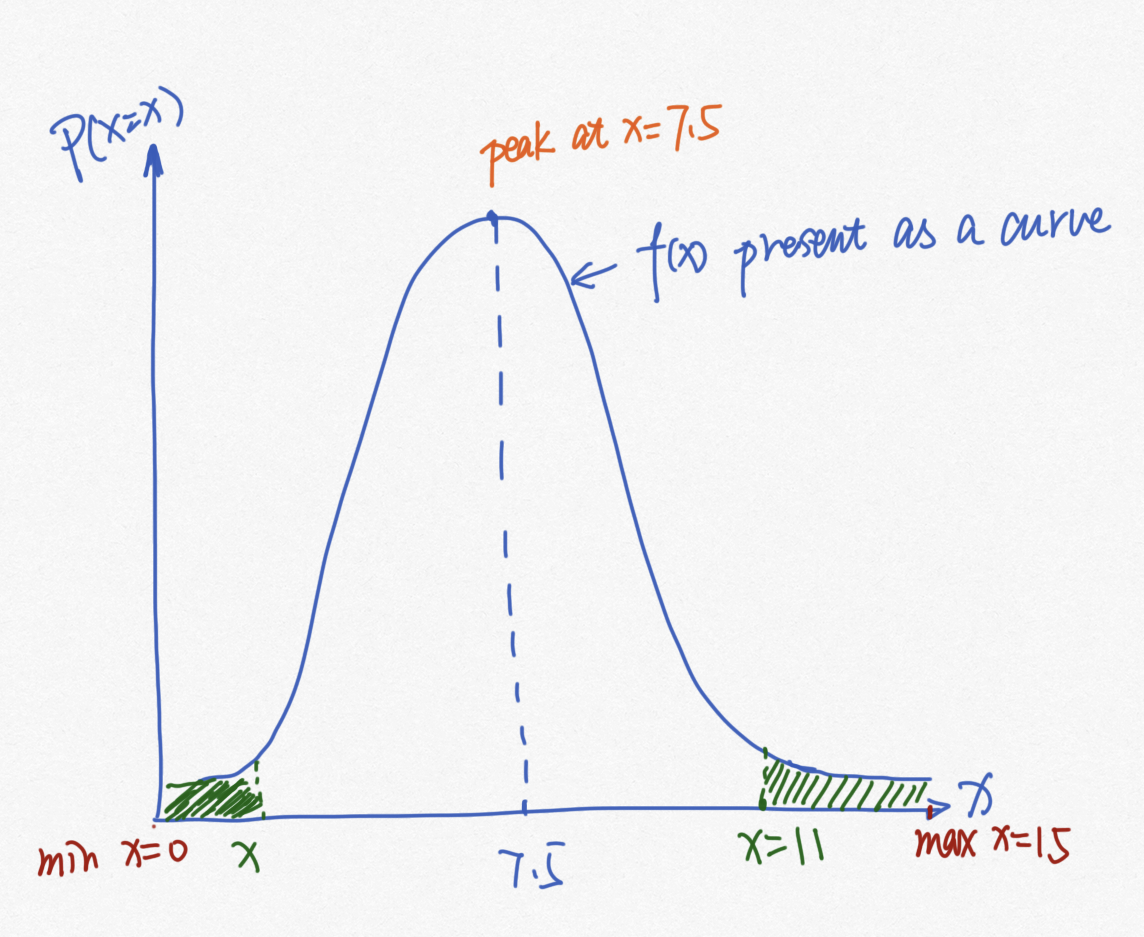
\includegraphics[width=0.8\linewidth]{q1c}
	\caption{shape of probability function of $X$ under null hypothesis}
	\label{fig:q1c}
\end{figure}
			\item For the $p$-value: \begin{align*}
				\mathbb{P}(X \geq 11) & = 1 - \mathbb{P}(X < 11) \\
				& = 1 - \mathbb{P}(X \leq 10) \\
				& = 1 - F_X(10)
			\end{align*}
			The $R$ code for the $p$-value is: \quad \texttt{2 * (1 - pbinom(10,15,0.5))}\\
			$p$-value is calculated as $0.12$. If the true probability is $0.5$, we have close to $12\%$ of the chance to see that out of $15$ races, team $A$ will win $11$ times. The $p$-value is big, therefore we don't have evidence against of null hypothesis. The null hypothesis just to test whether the winning probability is $0.5$ and we don't have evidence that Team $A$ is quicker than Team $B$.
			\item If team $A$ won $110$ out of $150$ times, and conducting the same test, the $p$-value will become smaller than we will have more evidence against $H_0$. It's because the more samples we have, the less uncertainty about the population, and the probability will get more close to the true parameter, and less probability that our observed outcome just by chance.  If our true probability is $0.5$, when the sample is big as $150$, we are expected to see that team $A$ and team $B$ will win roughly the  same amount of number. Since out of $150$ races, team $A$ won $110$ times, it's more likely that team $A$ has higher winning probability. 
		\end{enumerate}
		\item \begin{enumerate}[label = (\alph*)]
			\item $X$ is the number of customer who do not switch to a chocolate fish(failure) before $16$ chocolate finish has been used up(success) with probability $p$. The distribution of $X$ is negative binomial. \begin{align*}
				X \sim \text{Negative Binomial}(16, p)
			\end{align*}
			\item $X$ is \# of failures before $16$ chocolate fishes have been used up, total number of customer that has been ask is $25$, so the number of failure is $x = 25-16 = 9$\\
			 \begin{align*}
			 L(p;9) & = P(X = 9) \text{ when } X \sim \text{NegBin}(16,p)\\
				L(p;9) & = \binom{16+9-1}{9}p^{16}(1-p)^9 = \binom{24}{9} p^{16}(1-p)^9 \qquad \text{for } 0 < p < 1
			\end{align*} 
			
			
			When $\cfrac{dL}{dp} = 0$, the probability is maximum. 
			 \begin{align*}
			 \cfrac{dL}{dp}& = \binom{24}{9}\left(16p^{15}(1-p)^9 + p^{16}\times 9 \times (1-p)^{8}\times (-1)\right) \quad \text{product rule} \\
			 & = \binom{24}{9}p^{15}(1-p)^{8}\left(16(1-p) - 9p\right) \\
			 & = \binom{24}{9}p^{15}(1-p)^{8}(16 - 25p) \quad \text{for } 0 < p < 1\\
			 \text{ when } \left.\cfrac{dL}{dp} \right |_{p = \hat{p}}&= 0 \\
			 &\implies\binom{24}{9}\hat{p}^{15}(1-\hat{p})^{8}(16 - 25\hat{p})  = 0 \\
			 &\implies \hat{p} = 0 \text{ or } \hat{p} = 1 \text{ or } 16 - 25\hat{p} = 0
			 \end{align*}
			According the likelihood function of graph does dot peak at  $\hat{p} = 0$ or $\hat{p} = 1$, the peak is close to $0.6$.
			Maximizing $L$ with respect to $p$ to find $MLE$ when $x = 9$, $16 - 25\hat{p} = 0 \implies \hat{p} =  \cfrac{16}{25} = 0.64$
			\item 
			when observed $X = x$, The maximum likelihood function for $0 < p < 1$ is given below
			\begin{align*}
			L(p;x) & = P(X = x) \text{ when } X \sim \text{NegBin}(16,p)\\
			L(p;x) & = \binom{16+x-1}{x}p^{16}(1-p)^x \\
			& = \binom{15+x}{x} p^{16}(1-p)^x \qquad \text{for } 0 < p < 1
			\end{align*}
			When $\cfrac{dL}{dp} = 0$, the value is at its maximum.We first calculate $\cfrac{dL}{dp}$
			\begin{align*}
			\cfrac{dL}{dp}& = \binom{15 +x}{x}\left(16p^{15}(1-p)^x + p^{16}\times x(1-p)^{x-1}\times (-1)\right) \quad \text{product rule} \\
			& = \binom{15+x}{9}p^{15}(1-p)^{x-1}\left(16(1-p) - xp\right) \\
			& = \binom{15+x}{9}p^{15}(1-p)^{x-1}(16 - (16+x)p) \quad \text{for } 0 < p < 1
			\end{align*}
			Then, we calculate $\left.	\cfrac{dL}{dp}\right | _{p = \hat{p}} = 0$
			\begin{align*}
			\left.	\cfrac{dL}{dp}\right | _{p = \hat{p}} & = \binom{15+x}{9}\hat{p}^{15}(1-\hat{p})^{x-1}(16 - (16+x)\hat{p}) = 0 \\
			& \implies 16 - (16+x)\hat{p} = 0 \\
			\implies \hat{p} & = \cfrac{16}{16+x}
			\end{align*}
			
			
			We know that the $MLE$ of $L$ with respect to $p$ is $\hat{p}  = \cfrac{16}{16+x}$. 
			Replace $x$ with $X$, we will get the estimator $\hat{p} = \cfrac{16}{16+X}$
			\item $X$ has negative binomial distribution with probability of $p$, \begin{align*}
			X  \sim &\text{Negative Binomial}(16, p)\\
			H_0: &p = 0.5 \\
			H_1: & p \neq 0.5 \qquad \text{(two-sided test)}
			\end{align*}
			\item $f_X(x) = \binom{16+x-1}{x}p^{16}(1-p)^x$, under null hypothesis, $p = 0.5$\\
			$p_1 = \mathbb{P}(X=9) = \binom{16+9-1}{x}p^{16}(1-p)^9 =0.0390\\
			p_2 =\mathbb{P}(X=25) = \binom{16+25-1}{x}p^{16}(1-p)^{25} =  0.0183$
			\item $p$-value is the probability of getting a result at least as extreme as $X = 9$. And results at least as extrem as $X = 9$ are $X \leq  9 $ and the equal probability in the opposite direction. \\
			We know that $\mathbb{P}(X\leq 9) = 0.1148$, so the $p$-value = $2 \times\mathbb{P}(X\leq 9) =  0.2296$\\
			The data is compatible with $H_0$, we don't have evidence to against our null hypothesis which is that the probability of each customer switching the the chocolate fish is the same as not switching. Catriona's suspicion is not been justified. 
		\end{enumerate}
		\item \begin{enumerate}[label = (\alph*)]
			\item Each variable $Y_i$ is independent, and each variable has distribution $Y_i \sim \text{Poisson}(\beta \log(x_i))$\\
			$\mathbb{E}(Y_i) = \beta \log(x_i)$\\
			$\text{Var}(Y_i) = \mathbb{E}(Y_i) = \beta \log(x_i)$
			\item Using Matiu's model, $Y_1, Y_2, Y_3 Y_4$ are independent, then we have 
			\[\mathbb{P}(Y_1 = y_1, Y_2 = y_2, Y_3 = y_3,Y_4 = y_4) = \mathbb{P}(Y_1 = y_1)\mathbb{P}(Y_2 = y_2)\mathbb{P}(Y_3 = y_3)\mathbb{P}(Y_4 = y_4)\]
			So, we could write 
			\[\mathbb{P}(Y_1 = 329, Y_2 = 437, Y_3 = 590,Y_4 = 630) = \mathbb{P}(Y_1 = 329)\mathbb{P}(Y_2 = 437)\mathbb{P}(Y_3 = 590)\mathbb{P}(Y_4 = 630)\]
			\item The likelihood function is \begin{align*}
				L(\beta; y,x) & = \mathbb{P}(y_1,y_2,y_3,y_4|x_1,x_2,x_3,x_4;\beta) \\
				& =  \prod_{i = 1}^{4}\mathbb{P}(y_i|x_i ; \beta) \qquad (\text{by independence}) \\
				& = \prod_{i = 1}^{4}\cfrac{(\beta \log(x_i))^{y_i}}{y_i!}e^{-\beta \log(x_i)}\\
				& =  \prod_{i = 1}^{4}(\cfrac{\log(x_i)^{y_i}}{y_i!})\beta^{y_i}e^{-\beta \log(x_i)} \\
				& = K \beta^{y_1 + y_2 + y_3 + y_4}e^{-\beta(\log(x_1) + \log(x_2) + \log(x_3) + \log(x_4))} \\
				& = K \beta^{y_1 + y_2 + y_3 + y_4}e^{-\beta\log(x_1x_2x_3x_4)} \quad \text{where K is a constant not depend on } \beta\\
				& \text{ for } 0<\beta < \infty
			\end{align*}
			\item In order to find the maximum value for $\beta$, we differentiate likelihood function and set to $0$ for $MLE$. 
			\begin{align*}
				0 & = \cfrac{d}{d\beta}L(\beta; y_1,y_2,y_3,y_4)\\
				& = \cfrac{d}{d\beta}\{K \beta^{y_1 + y_2 + y_3 + y_4}e^{-\beta\log(x_1x_2x_3x_4)}\} \\
				& = K((y_1 + y_2 + y_3 + y_4)\beta^{y_1 + y_2 + y_3 + y_4-1}e^{-\beta\log(x_1x_2x_3x_4)}\\
				 & - \beta^{y_1 + y_2 + y_3 + y_4}\log(x_1x_2x_3x_4)e^{-\beta\log(x_1x_2x_3x_4)}) \\
				 & = K\beta^{y_1 + y_2 + y_3 + y_4-1}e^{-\beta\log(x_1x_2x_3x_4)}((y_1 + y_2 + y_3 + y_4)-\beta\log(x_1x_2x_3x_4) )\\
				 \implies 0 & = (y_1 + y_2 + y_3 + y_4)-\beta\log(x_1x_2x_3x_4) \quad \text{ or } \beta = 0, \infty \\
				 \implies \hat{\beta} & = \cfrac{y_1 + y_2 + y_3 + y_4}{\log(x_1x_2x_3x_4)} \quad \text{assuming a unique maximum in } 0< \beta < \infty
			\end{align*}
		To obtain maximum likelihood estimator, just replace $y_i$ with variable $Y_i$\\
		\[\hat{\beta}  = \cfrac{Y_1 + Y_2 + Y_3 + Y_4}{\log(x_1x_2x_3x_4)} \]
			\item The $MLE$ is \begin{align*}
				\hat{\beta} & =  \cfrac{329 + 437 + 590+ 630}{\log(50\times 100 \times 150 \times 200)} \\
				& = 105.4916
			\end{align*}
			\item \begin{align*}
				\mathbb{E}(\hat{\beta}) & = \mathbb{E}\left(\cfrac{Y_1 + Y_2 + Y_3 + Y_4}{\log(x_1x_2x_3x_4)}\right) \\
				& = \cfrac{1}{\log(x_1x_2x_3x_4)}\mathbb{E}(Y_1 + Y_2 + Y_3 + Y_4) \\
				& = \cfrac{1}{\log(x_1x_2x_3x_4)}\left( \mathbb{E}(Y_1) +\mathbb{E}(Y_2)+\mathbb{E}(Y_3)+\mathbb{E}(Y_4)\right) \\
				& =  \cfrac{1}{\log(x_1x_2x_3x_4)}\left(\beta \log(x_1)+\beta \log(x_2)+\beta \log(x_3)+\beta \log(x_4)\right)\\
				& = \beta  \cfrac{1}{\log(x_1x_2x_3x_4)}\times \log(x_1x_2x_3x_4)\\
				& = \beta
			\end{align*}
			We derived our case that $\mathbb{E}(\hat{\beta}) = \beta$, so $\hat{\beta}$ is an unbiased estimator.
			\item \begin{align*}
				\mathbb{E}(Z_i) & = \mathbb{E}(Y_i - x_i)\\
				& = \mathbb{E}(Y_i) - \mathbb{E}(x_i)\\
				& = \beta \log(x_i) - x_i
			\end{align*}
		\end{enumerate}
	\end{enumerate}
\end{document}